\documentclass{beamer}
\usetheme{Boadilla}
\usecolortheme{dolphin}
\usefonttheme{serif}
\setbeamertemplate{navigation symbols}{}
\setbeamertemplate{caption}[numbered]
\usepackage{graphicx}
\usepackage{amsmath}
\usepackage{hyperref}
\usepackage{booktabs}
\usepackage{multicol}
\usepackage{pgfplots}
\pgfplotsset{compat=1.18}

\title{An Economic Analysis of Optimal Investment Strategies for Accumulating Housing Down Payments}
\author{Frank Paul Longo II}
\date{\today}

\begin{document}

\begin{frame}
    \titlepage
\end{frame}

\begin{frame}{Overview}
    \tableofcontents
\end{frame}

\section{Introduction}
\begin{frame}{Introduction}
    \begin{block}{Objective}
        Develop investment strategies for first-time homebuyers to save for down payments.
    \end{block}
    \begin{block}{Research Question}
        What are the best strategies for different age groups to save for down payments in 5, 10, and 15 years?
    \end{block}
    \begin{block}{Motivation}
        Address challenges from rising housing costs and help diverse age groups accelerate homeownership.
    \end{block}
\end{frame}



\section{Literature Review}
\begin{frame}{Markowitz (1952)}
    \begin{block}{Key Concepts}
        Introduction of Modern Portfolio Theory (MPT)
    \end{block}
    \begin{block}{Contribution}
        Markowitz's work laid the foundation for constructing portfolios that optimize the trade-off between risk and return.
    \end{block}
    \begin{block}{Application}
        \begin{itemize}
            \item Provides the framework for constructing efficient portfolios.
            \item Essential for developing strategies that balance risk and return.
            \item Helps identify optimal portfolio mixes that maximize return for a given risk level.
        \end{itemize}
    \end{block}
\end{frame}


\begin{frame}{Sharpe (1966)}
    \begin{block}{Key Concepts}
        Development of the Sharpe Ratio
    \end{block}
    \begin{block}{Contribution}
        Introduced a method to measure the risk-adjusted return of an investment.
    \end{block}
    \begin{block}{Application}
        \begin{itemize}
            \item Critical for evaluating and comparing different investment strategies.
            \item Helps identify investments with the best returns relative to their risk.
            \item Enables comparison of portfolio performance on a risk-adjusted basis.
        \end{itemize}
    \end{block}
\end{frame}


\begin{frame}{Boyle (1977)}
    \begin{block}{Key Concepts}
        Introduction of Monte Carlo methods for pricing options
    \end{block}
    \begin{block}{Contribution}
        Demonstrated the application of Monte Carlo simulation for complex financial derivatives.
    \end{block}
    \begin{block}{Application}
        \begin{itemize}
            \item Provides a framework for using Monte Carlo simulations in financial modeling.
            \item Models the uncertainty and variability of investment returns over time.
            \item Supports the development of probabilistic models to simulate the accumulation of down payments.
        \end{itemize}
    \end{block}
\end{frame}


\section{Typical First-time Homebuyer Profile}
\begin{frame}{Typical First-time Homebuyer Profile}
    \begin{block}{Demographics}
        \begin{itemize}
            \item \textbf{Average Age:} 35 years (2023)
            \item \textbf{Median Income:} \$95,900 (2023)
        \end{itemize}
    \end{block}
    \begin{block}{Marital Status}
        \begin{itemize}
            \item 59\% Married Couples
            \item 19\% Single Females
            \item 10\% Single Males
            \item 9\% Unmarried Couples
        \end{itemize}
    \end{block}
    \begin{block}{Financials}
        \begin{itemize}
            \item \textbf{Average Home Cost:} \$348,000 (2022) 
            \item \textbf{Down Payment Saved:} \$8,220 
        \end{itemize}
    \end{block}
\end{frame}


\section{Risk Tolerances and Investment Contributions}
\begin{frame}{Investment Contributions by Age Group}
    \begin{block}{Data Source}
        Bureau of Labor Statistics (BLS), Federal Reserve
    \end{block}
    \begin{block}{Annual Income and Contributions}
        \begin{itemize}
            \item \textbf{20-25 years:} 
            \begin{itemize}
                \item Median income: \$45,000
                \item Annual contribution: 10\% of income
            \end{itemize}
            \item \textbf{25-30 years:} 
            \begin{itemize}
                \item Median income: \$60,000
                \item Annual contribution: 15\% of income
            \end{itemize}
            \item \textbf{30-35 years:} 
            \begin{itemize}
                \item Median income: \$80,000
                \item Annual contribution: 20\% of income
            \end{itemize}
        \end{itemize}
    \end{block}
\end{frame}



\section{Data Sources and Analysis}
\begin{frame}{Data Sources and Analysis}
    \begin{block}{Primary Source}
        \textbf{Yahoo Finance (YFinance)}
        \begin{itemize}
            \item Comprehensive financial data on stocks, cryptocurrency, mutual funds, and ETFs.
        \end{itemize}
    \end{block}
    \begin{block}{Data Coverage}
        \textbf{Date Range:} 9/7/2014 to present (daily frequency)
    \end{block}
    \begin{block}{Data Fields}
        \begin{multicols}{2}
        \begin{itemize}
            \item Open
            \item High
            \item Low
            \item Close
            \item Adj Close
            \item Volume
            \item Type
        \end{itemize}
        \end{multicols}
    \end{block}
\end{frame}



\section{Financial Literacy: Essential Concepts}
\begin{frame}{Essential Financial Concepts}
    \begin{block}{Stocks}
        Equity investments representing ownership in a company.
    \end{block}
    \begin{block}{Cryptocurrency}
        Digital or virtual currencies that use cryptography for security.
    \end{block}
    \begin{block}{Mutual Funds}
        Investment vehicles that pool money from many investors to purchase a diversified portfolio of stocks, bonds, or other securities.
    \end{block}
    \begin{block}{ETFs (Exchange-Traded Funds)}
        Similar to mutual funds but traded on stock exchanges like individual stocks.
    \end{block}
\end{frame}


\section{CAPM and Sharpe Ratio}
\begin{frame}{Capital Asset Pricing Model (CAPM)}
    \begin{block}{Formula} 
        \begin{equation*}
            E(R_i) = R_f + \beta_i (E(R_m) - R_f)
        \end{equation*}
    \end{block}
    \begin{block}{Assumptions}
        \begin{itemize}
            \item Diversified portfolios
            \item Efficient markets
            \item No taxes or transaction costs
            \item Constant risk-free rate
        \end{itemize}
    \end{block}
\end{frame}


\begin{frame}{Calculating CAPM}
    \begin{block}{Step 1: Identify Risk-Free Rate}
        \begin{equation*}
            R_f = 3\%
        \end{equation*}
    \end{block}
    \begin{block}{Step 2: Determine Market Return}
        \begin{equation*}
            E(R_m) = 8\%
        \end{equation*}
    \end{block}
    \begin{block}{Step 3: Calculate Asset Beta}
        \begin{equation*}
            \beta_i = \frac{\text{Cov}(R_i, R_m)}{\sigma_m^2}
        \end{equation*}
    \end{block}
    \begin{block}{Step 4: Calculate Expected Return}
        \begin{equation*}
            E(R_i) = 3\% + 0.75 (8\% - 3\%) = 6.75\%
        \end{equation*}
    \end{block}
\end{frame}


\begin{frame}{Sharpe Ratio}
    \begin{block}{Purpose}
        Measures investment performance adjusted for risk.
    \end{block}
    \begin{block}{Formula}
        \begin{equation*}
            S = \frac{E(R_i) - R_f}{\sigma_i}
        \end{equation*}
    \end{block}
    \begin{block}{Components}
        \begin{itemize}
            \item \(E(R_i)\): Expected return
            \item \(R_f\): Risk-free rate
            \item \(\sigma_i\): Std. deviation of excess return
        \end{itemize}
    \end{block}
    \begin{block}{Interpretation}
        \begin{itemize}
            \item Higher ratio = better performance
        \end{itemize}
    \end{block}
\end{frame}





\begin{frame}{Calculating Sharpe Ratio}
    \begin{block}{Step 1: Calculate Expected Return (from CAPM)}
        \begin{equation*}
            E(R_i) = 6.75\%
        \end{equation*}
    \end{block}
    \begin{block}{Step 2: Identify Risk-Free Rate}
        \begin{equation*}
            R_f = 3\%
        \end{equation*}
    \end{block}
    \begin{block}{Step 3: Determine Standard Deviation of Asset}
        \begin{equation*}
            \sigma_i = 10\%
        \end{equation*}
    \end{block}
    \begin{block}{Step 4: Calculate Sharpe Ratio}
        \begin{equation*}
            S = \frac{6.75\% - 3\%}{10\%} = 0.375
        \end{equation*}
    \end{block}
\end{frame}


\begin{frame}{Security Market Line (SML)}
    \begin{figure}[h]
        \centering
        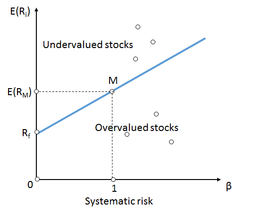
\includegraphics[width=\textwidth]{SML.png}
    \end{figure}
\end{frame}


\section{Modern Portfolio Theory (MPT)}
\begin{frame}{Modern Portfolio Theory (MPT)}
    \begin{block}{Overview}
        Framework for constructing a portfolio to maximize return for a given level of risk.
    \end{block}
    \begin{block}{Formulas}
        \begin{equation*}
            E(R_p) = \sum_{i=1}^{n} w_i E(R_i)
        \end{equation*}
        \begin{equation*}
            \sigma_p^2 = \sum_{i=1}^{n} \sum_{j=1}^{n} w_i w_j \sigma_{ij}
        \end{equation*}
    \end{block}
    \begin{block}{Definitions}
        \begin{multicols}{2}
            \begin{itemize}
                \item \(E(R_p)\): Portfolio return
                \item \(w_i\): Weight of asset \(i\)
                \item \(E(R_i)\): Return of asset \(i\)
                \item \(\sigma_p^2\): Portfolio variance
                \item \(\sigma_{ij}\): Covariance of assets \(i, j\)
            \end{itemize}
        \end{multicols}
    \end{block}
\end{frame}










\begin{frame}{Step 1: Define Assets and Expected Returns}
    \begin{block}{Identify Assets}
        Choose the assets to include in the portfolio.
    \end{block}
    \begin{block}{Estimate Expected Returns}
        Calculate the expected returns (\(E(R_i)\)) for each asset.
        \begin{equation*}
            E(R_i) = \text{Expected return of asset } i
        \end{equation*}
    \end{block}
    \begin{block}{Example}
        \begin{itemize}
            \item Asset A: \(E(R_A) = 10\%\)
            \item Asset B: \(E(R_B) = 15\%\)
        \end{itemize}
    \end{block}
\end{frame}



\begin{frame}{Step 2: Determine Asset Weights}
    \begin{block}{Decide Proportions}
        Allocate the proportion (\(w_i\)) of the total investment to each asset.
    \end{block}
    \begin{block}{Constraint}
        The sum of the weights should equal 1.
        \begin{equation*}
            \sum_{i=1}^{n} w_i = 1
        \end{equation*}
    \end{block}
    \begin{block}{Example}
        \begin{itemize}
            \item Weight of Asset A: \(w_A = 60\%\)
            \item Weight of Asset B: \(w_B = 40\%\)
        \end{itemize}
    \end{block}
\end{frame}


\begin{frame}{Step 3: Calculate Portfolio's Expected Return}
    \begin{block}{Formula}
        The expected return of the portfolio (\(E(R_p)\)) is the weighted sum of the expected returns of the individual assets.
        \begin{equation*}
            E(R_p) = \sum_{i=1}^{n} w_i E(R_i)
        \end{equation*}
    \end{block}
    \begin{block}{Example Calculation}
        \begin{equation*}
            E(R_p) = (0.60 \times 0.10) + (0.40 \times 0.15) = 0.12 \text{ or 12\%}
        \end{equation*}
    \end{block}
\end{frame}


\begin{frame}{Step 4: Calculate Covariances Between Assets}
    \begin{block}{Definition}
        Covariance measures how two assets move together.
    \end{block}
    \begin{block}{Interpretation}
        \begin{itemize}
            \item Positive covariance: Assets tend to move in the same direction.
            \item Negative covariance: Assets tend to move in opposite directions.
        \end{itemize}
    \end{block}
    \begin{block}{Formula}
        \begin{equation*}
            \sigma_{ij} = \text{Cov}(R_i, R_j) = \mathbb{E}[(R_i - \mathbb{E}[R_i])(R_j - \mathbb{E}[R_j])]
        \end{equation*}
    \end{block}
    \begin{block}{Example}
        Covariance between Asset A and Asset B: \(\sigma_{AB} = 0.02\)
    \end{block}
\end{frame}


\begin{frame}{Step 5: Calculate Portfolio's Variance (Risk)}
    \begin{block}{Formula}
        The variance (\(\sigma_p^2\)) of the portfolio's return is determined by the variances of the individual assets and the covariances between them.
        \begin{equation*}
            \sigma_p^2 = \sum_{i=1}^{n} \sum_{j=1}^{n} w_i w_j \sigma_{ij}
        \end{equation*}
    \end{block}
    \begin{block}{Example Calculation}
        \begin{equation*}
            \sigma_p^2 = (0.60)^2 \times 0.04 + (0.40)^2 \times 0.09 + 2 \times 0.60 \times 0.40 \times 0.02 = 0.0384
        \end{equation*}
    \end{block}
\end{frame}


\begin{frame}{Step 6: Optimize the Portfolio}
    \begin{block}{Objective}
        Adjust the weights of the assets to maximize the portfolio's expected return for a given level of risk or to minimize risk for a given level of expected return.
    \end{block}
    \begin{block}{Optimization Problem}
        Solve the following optimization problem:
        \begin{equation*}
            \min \sigma_p^2 = \sum_{i=1}^{n} \sum_{j=1}^{n} w_i w_j \sigma_{ij}
        \end{equation*}
        Subject to:
        \begin{equation*}
            \sum_{i=1}^{n} w_i = 1 \quad \text{and} \quad E(R_p) = \sum_{i=1}^{n} w_i E(R_i)
        \end{equation*}
    \end{block}
\end{frame}


\begin{frame}{Efficient Frontier}
    \begin{figure}[h]
        \centering
        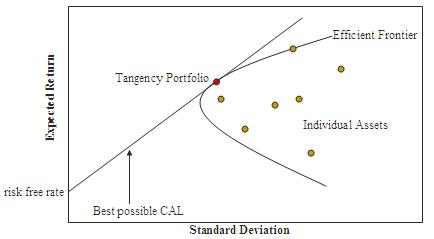
\includegraphics[width=\textwidth]{efficient_frontier.png}
        \caption{Efficient Frontier}
    \end{figure}
\end{frame}


\section{Monte Carlo Simulation}
\begin{frame}{Monte Carlo Simulation: Purpose and Theory}
    \begin{block}{Purpose}
        Model the probability of different outcomes by incorporating randomness and uncertainty.
    \end{block}
    \begin{block}{Mathematical Theory}
        \begin{itemize}
            \item \textbf{Random Sampling:} Generate random variables \(X_i\) based on the historical return distribution.
            \item \textbf{Simulation Process:}
            \begin{equation*}
                X_i = X_{i-1} \times (1 + r_i)
            \end{equation*}
            where \(r_i\) is the return for period \(i\).
        \end{itemize}
    \end{block}
\end{frame}

\begin{frame}{Monte Carlo Simulation: Calculation and Definitions}
    \begin{block}{Expected Value Calculation}
        \begin{equation*}
            \text{E}(X) = \frac{1}{N} \sum_{i=1}^{N} X_i
        \end{equation*}
    \end{block}
    \begin{block}{Risk Assessment}
        Analyze the distribution of simulated outcomes to understand the range of possible investment values.
    \end{block}
    \begin{block}{Definitions}
        \begin{itemize}
            \item \( \text{E}(X) \): Expected value of the outcome
            \item \( N \): Number of simulations
            \item \( X_i \): Simulated variable
        \end{itemize}
    \end{block}
\end{frame}







\begin{frame}{Monte Carlo Simulation Example}
    \begin{block}{Example Purpose}
        Simulate investment returns over 5, 10, and 15 years to assess the probability of accumulating sufficient funds for a down payment.
    \end{block}
    \begin{block}{Steps}
        \begin{enumerate}
            \item Define initial investment and annual contribution.
            \item Generate random returns based on historical data.
            \item Repeat the simulation multiple times to estimate the distribution of outcomes.
        \end{enumerate}
    \end{block}
\end{frame}



\section{Conclusion}
\begin{frame}{Conclusion}
    \begin{block}{Future Directions}
        Explore optimal investment strategies tailored for first-time homebuyers to accumulate housing down payments, incorporating modern financial theories and data-driven insights.
    \end{block}
    \begin{block}{Effective Strategies}
        \begin{itemize}
            \item Diversified portfolios
            \item Application of Modern Portfolio Theory (MPT)
            \item Lifecycle investing to navigate unique financial challenges
        \end{itemize}
    \end{block}
    \begin{block}{Ongoing Research}
        Focus on refining these strategies and exploring their practical applications to further assist first-time homebuyers in achieving their homeownership goals.
    \end{block}
\end{frame}


\begin{frame}{Q\&A}
    \begin{block}{Questions and Clarifications}
        Please feel free to ask for any clarifications or additional details regarding the presented research and findings.
    \end{block}
    \vspace{1cm}
    \begin{center}
        \Large \textbf{Thank you for your attention!}
    \end{center}
\end{frame}


\begin{frame}{References (1/2)}
    \begin{itemize}
        \item Yahoo Finance. (n.d.). Retrieved from \url{https://finance.yahoo.com/}
        \item Robinhood. (n.d.). Retrieved from \url{https://robinhood.com/}
        \item Coinbase. (n.d.). Retrieved from \url{https://www.coinbase.com/}
        \item Investment Company Institute. (n.d.). Retrieved from \url{https://www.ici.org/}
    \end{itemize}
    \begin{itemize}
        \item Sharpe, W. F. (1966). Mutual Fund Performance. \textit{Journal of Business, 39}(1), 119-138. DOI: 10.1086/294846
        \item Markowitz, H. (1952). Portfolio Selection. \textit{Journal of Finance, 7}(1), 77-91. DOI: 10.2307/2975974
        \item Boyle, P. P. (1977). Options: A Monte Carlo Approach. \textit{Journal of Financial Economics, 4}(3), 323-338. DOI: 10.1016/0304-405X(77)90005-8
    \end{itemize}
\end{frame}

\begin{frame}{References (2/2)}
    \begin{itemize}
        \item National Association of Realtors. (2023). 2023 Home Buyer and Seller Generational Trends. Retrieved from \url{https://www.nar.realtor/research-and-statistics/research-reports/home-buyer-and-seller-generational-trends}
        \item Federal Reserve. (2023). Report on the Economic Well-Being of U.S. Households in 2023. Retrieved from \url{https://www.federalreserve.gov/publications/2023-economic-well-being-of-us-households-in-2023.htm}
        \item Bureau of Labor Statistics (BLS). (2023). Income and Expenditures. Retrieved from \url{https://www.bls.gov/income-and-expenditures.htm}
    \end{itemize}
\end{frame}

\end{document}
